Outlined below are some coding fragments categorised under: Design Patterns, Asynchronous Tasks, Presenters, Views and Interesting Coding Fragments.

\tocless\subsection{Design Patterns}
Various design patterns were used in the implementation of this application such as the Factoy, the Builder and the Singleton which are outlined below.

The Factory design pattern was used to retrieve a DAO (Data Access Object) as seen in Figure \ref{lst:daoFactory}.
This was used so that if at a future time the storage type of the application is to be changed, the developer would only have to change one instance of the codebase and return a new implementation of the DAO interface in the method getDAO().
\begin{figure}[h]
\caption{DAO Factory Class}
\label{lst:daoFactory}
\begin{lstlisting}[style=Java]
public class DAOFactory {

    public DAO getDAO(Context context){
        return SqlLiteDAO.getInstance(context);
    }
}
\end{lstlisting}
\end{figure}

A Host builder was used to create a Host object.
This builder is a static inner class in the Host class file as documented in Figure \ref{lst:hostBuilder}
\begin{figure}[h]
\caption{HostBuilder Class}
\label{lst:hostBuilder}
\begin{lstlisting}[style=Java]
public static class HostBuilder {
    private final String ipv4;
    private String dns;
    private int port;
    private String route;

    public HostBuilder(String ipv4) {
        this.ipv4 = ipv4;
    }

    public HostBuilder withDns(String dns) {
        this.dns = dns;
        return this;
    }

    public HostBuilder withPort(int port) {
        this.port = port;
        return this;
    }

    public HostBuilder withRoute(String route) {
        this.route = route;
        return this;
    }

    public Host build() {
        return new Host(this);
    }

}
\end{lstlisting}
\end{figure}

A Singleton instance of the DAO implementation was used in this application.
This was mainly due to the best practice of keeping database access objects as singleton instances.
This class ca be seen in Figure \ref{lst:singletonDao}.

\begin{figure}[h]
\caption{Singleton DAO Object}
\label{lst:singletonDao}
\begin{lstlisting}[style=Java]
public static DAO getInstance(Context context) {
    if(instance == null) {
        instance = new SqlLiteDAO(context);
    }
    return instance;
}
\end{lstlisting}
\end{figure}

\tocless\subsection{Asynchronous Tasks}
Asynchronous Tasks in Android are used to run tasks in the background or are sometimes used to simply distribute processess off the main thread.
The AsyncTask class must be extended on creation of the background processes.
An AsyncTask was used to send the food image to the backend host as in Figure \ref{lst:rrCode}.
\begin{figure}[h]
\caption{UploadImage Class}
\label{lst:rrCode}
\begin{lstlisting}[style=Java]
@Override
protected String doInBackground(Void... params) {
    String result = "";
    OkHttpClient client = new OkHttpClient();
    String imageToSend = image;
    RequestBody requestBody = new MultipartBody.Builder()
            .setType(MultipartBody.FORM)
            .addFormDataPart("image", imageToSend)
            .build();

    Request request = new Request.Builder().url(host.getUrl())
            .post(requestBody).build();

    Response response = null;
    try {
        response = client.newCall(request).execute();
        result = response.body().string();
        response.body().close();
    } catch (IOException e) {
        e.printStackTrace();
    }

    return result;
}
\end{lstlisting}
\end{figure}

\tocless\subsection{Presenters}
In the MPV architecture as described earlier, the presenter for each activity contains all the logic for that view.
The presenter in Figure \ref{lst:pres} was tasked with creating intents to new activities (views).
\begin{figure}[h]
\caption{MainPresenter Class}
\label{lst:pres}
\begin{lstlisting}[style=Java]
public class MainPresenter {

    private Intent intent;
    private Context context;

    public MainPresenter(Context context) {
        this.context=context;
    }

    public void takePhoto() {
        intent = new Intent(context, CaptureImageActivity.class);
        context.startActivity(intent);
    }

    public void userLogs() {
        intent = new Intent(context, FoodLogsActivity.class);
        context.startActivity(intent);
    }

}
\end{lstlisting}
\end{figure}

\tocless\subsection{Views}
In the MPV archtecture that this application uses, the views are responsible for interacting directly with the user interface.
The view for the MainActivity in Figure \ref{lst:mainView} responds to button clicks and calls to its presenter to carry out the logic of the required task.
\begin{figure}[h]
\caption{MainActivity Class}
\label{lst:mainView}
\begin{lstlisting}[style=Java]
public class MainActivity extends AppCompatActivity {

    private MainPresenter mainPresenter;

    @Override
    protected void onCreate(Bundle savedInstanceState) {
        super.onCreate(savedInstanceState);
        setContentView(R.layout.activity_main);

        mainPresenter = new MainPresenter(this);
    }

    public void onClickTakePhoto(View view) {
        mainPresenter.takePhoto();
    }

    public void onClickUserLogs(View view) {
        mainPresenter.userLogs();
    }
}
\end{lstlisting}
\end{figure}

\tocless\subsection{Storage}
SqlLite was used for storing data in this application and the class that handled creation, input and output to this database implemented the DAO interface.
An interface for storage devices was created so that each implementation would have the ability to add food logs, retrieve food logs, delete food logs and remove the data store completely.
Thisis documented in Figure \ref{lst:daoInterface}.
\begin{figure}[h]
\caption{DAO Interface}
\label{lst:daoInterface}
\begin{lstlisting}[style=Java]
public interface DAO {
    void addFoodLog(FoodLog foodLog);
    List<FoodLog> getLogsByDay(Date date);
    List<FoodLog> getLogsByWeek(Date date);
    List<FoodLog> getLogsByMonth(Date date);
    void deleteFoodLogs(List<FoodLog> foodLogs);
    void deleteDb();
}
\end{lstlisting}
\end{figure}

The method in Figure \ref{lst:getLogs} was used to execute a query and return a List of FoodLog objects.
\begin{figure}[h]
\caption{Get Food Logs Per Date}
\label{lst:getLogs}
\begin{lstlisting}[style=Java]
@Override
private List<FoodLog> selectQuery(String query) {
        foodLogs = new ArrayList<>();
        Cursor resultSet = database.rawQuery(query, null);
        while(resultSet.moveToNext()) {
            try {
                foodLogs.add(new FoodLogImpl
                .FoodLogBuilder(resultSet.getString(1))
                .withId(resultSet.getInt(0))
                .withCalories(resultSet.getDouble(2))
                .withTimestamp(dateFormat
                    .parse(resultSet.getString(3)))
                .build());
            } catch (ParseException e) {
                e.printStackTrace();
            }
        }
    return foodLogs;
}
\end{lstlisting}
\end{figure}

\tocless\subsection{Interesting Coding Fragments}
Some interesting coding fragments are outlined below which merit inclusion in this report.

The method in Figure \ref{lst:encodeBitmap} was used to encode the image taken on the phone to a string.
This was used to send the image to the backend with minimal latency.
The bitmap size was also reduced as in line 8 to decrease response time also.
\begin{figure}[h]
\caption{Encode Bitmap to base64 String}
\label{lst:encodeBitmap}
\begin{lstlisting}[style=Java]
public String toBase64() {
    BitmapFactory.Options options = new BitmapFactory.Options();
    options.inSampleSize = 8;

    Bitmap imageBitmap = BitmapFactory.decodeFile(image.getAbsolutePath(), options);

    //resize image for faster upload to server
    Bitmap.createScaledBitmap(imageBitmap, 300, 400, false);
    
    ByteArrayOutputStream byteArrayOutputStream = new ByteArrayOutputStream();
    imageBitmap.compress(Bitmap.CompressFormat.PNG, 100, byteArrayOutputStream);
    byte[] byteArray = byteArrayOutputStream.toByteArray();

    return Base64.encodeToString(byteArray, Base64.DEFAULT);
}
\end{lstlisting}
\end{figure}

A map of strings to runnables was used to query the database for food logs as documented in Figure \ref{lst:map}.
This was used as the select query for the database had to dynamically change depending on how the food logs were being viewed, by day, week, or month.
\begin{figure}[h]
\caption{Map of Runnables}
\label{lst:map}
\begin{lstlisting}[style=Java]
listViewOptions = new HashMap<>();
listViewOptions.put("Day", () -> getLogsByDay());
listViewOptions.put("Week",() -> getLogsByWeek());
listViewOptions.put("Month", () -> getLogsByMonth());
\end{lstlisting}
\end{figure}

\tocless\subsection{User Interface}
User interface implementation as in Figures \ref{fig:gallery}, \ref{fig:ui2}, \ref{fig:ui3}, \ref{fig:ui5}, \ref{fig:ui8}, \ref{fig:ui6}, \ref{fig:ui7} and \ref{fig:delete}.

\begin{figure}
  \label{uiDesign1} 
  \begin{minipage}[b]{0.5\linewidth}
    \centering
    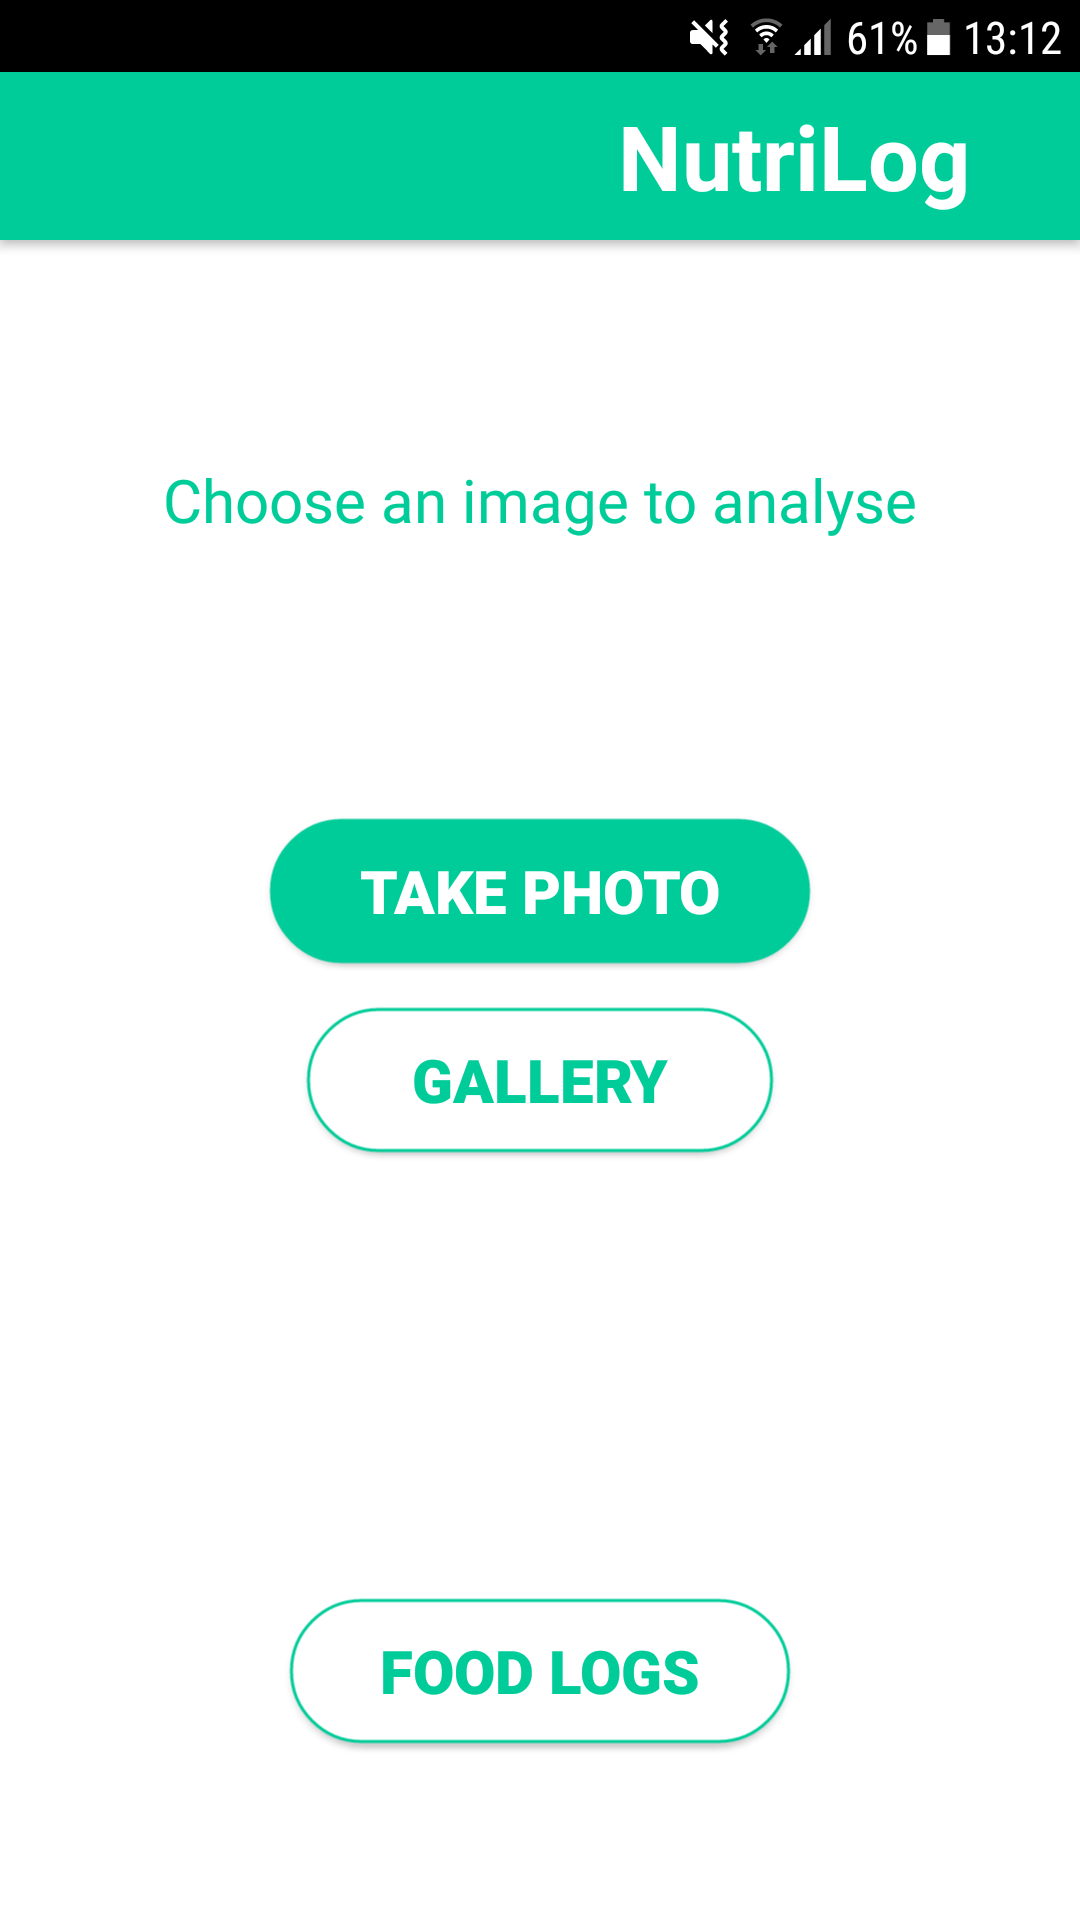
\includegraphics[width=.75\linewidth]{gallery} 
    \caption{Landing Activity} 
  \label{fig:gallery}
    \vspace{4ex}
  \end{minipage}%%
  \begin{minipage}[b]{0.5\linewidth}
    \centering
    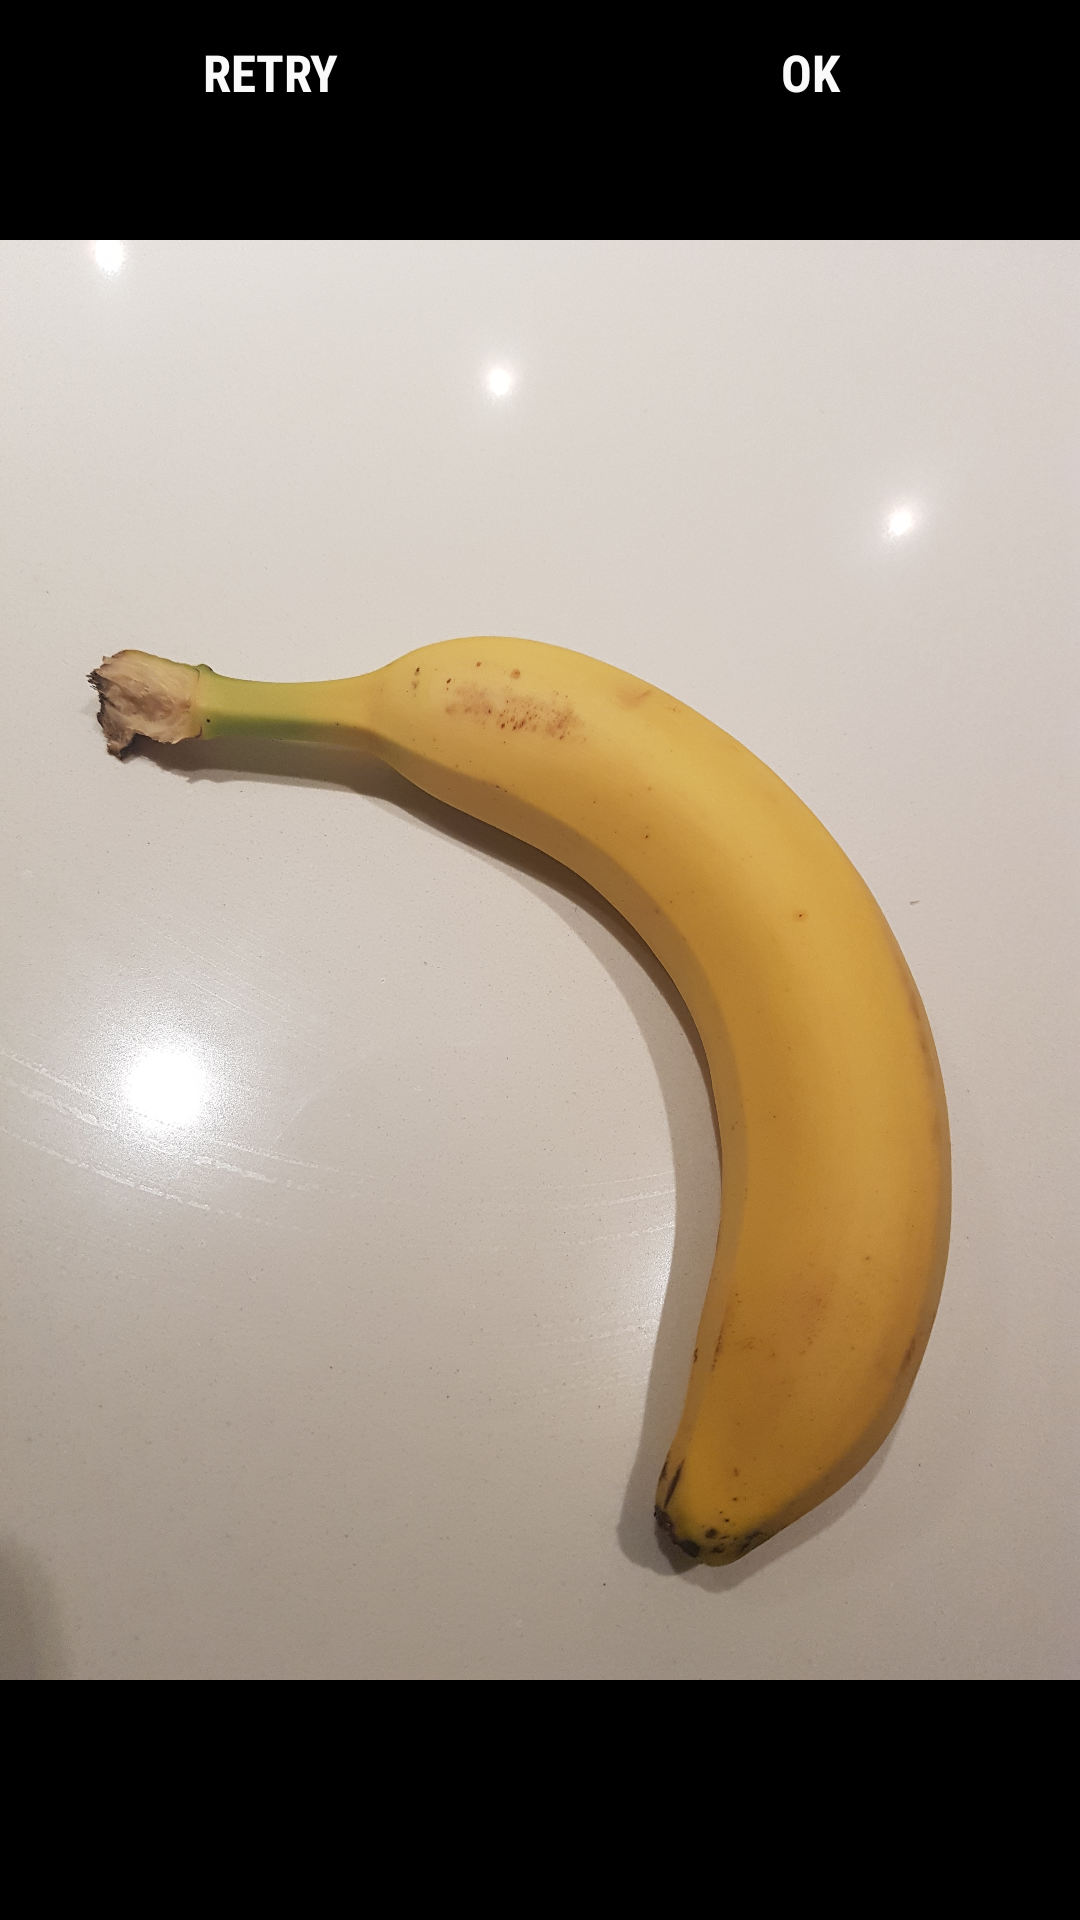
\includegraphics[width=.75\linewidth]{ui2} 
    \caption{Image Capture Activity} 
  \label{fig:ui2}
    \vspace{4ex}
  \end{minipage} 
  \begin{minipage}[b]{0.5\linewidth}
    \centering
    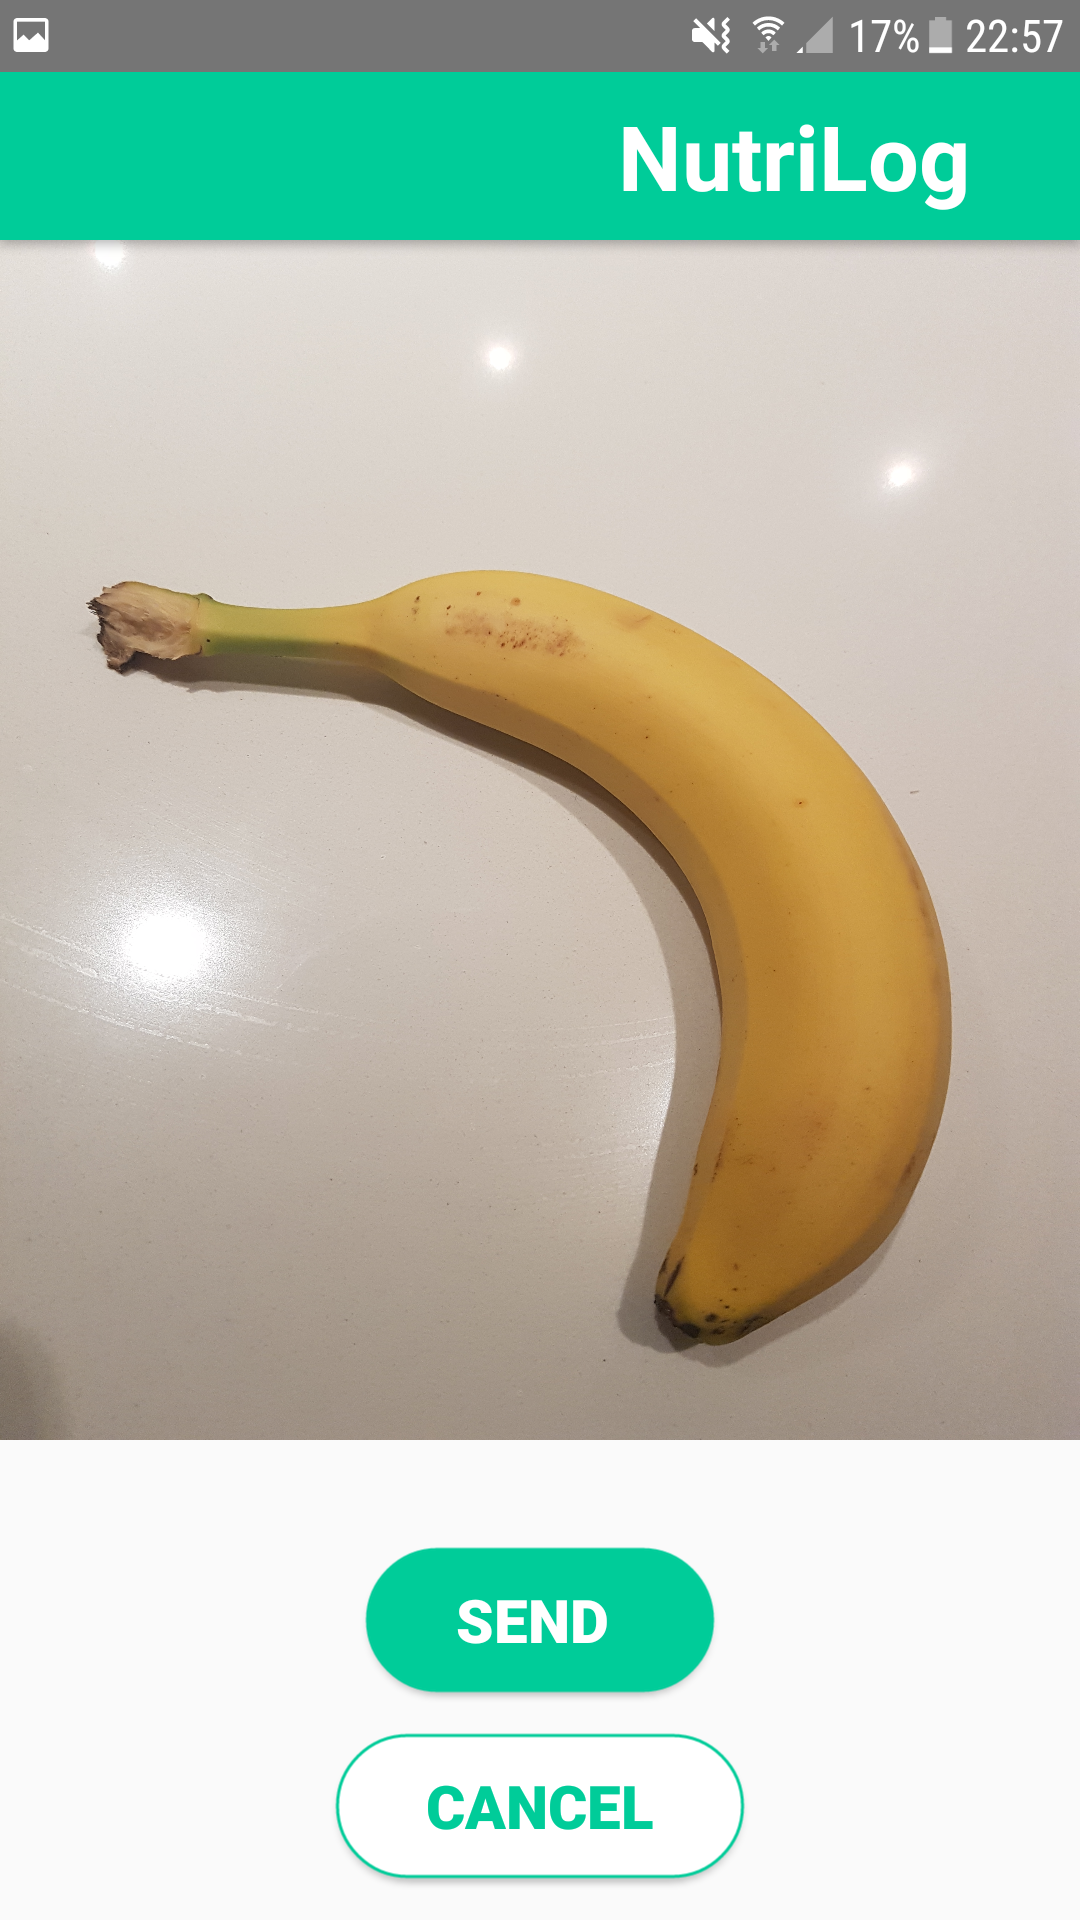
\includegraphics[width=.75\linewidth]{ui3} 
    \caption{Image Send Activity} 
    \label{fig:ui3}
    \vspace{4ex}
  \end{minipage}%% 
  \begin{minipage}[b]{0.5\linewidth}
    \centering
    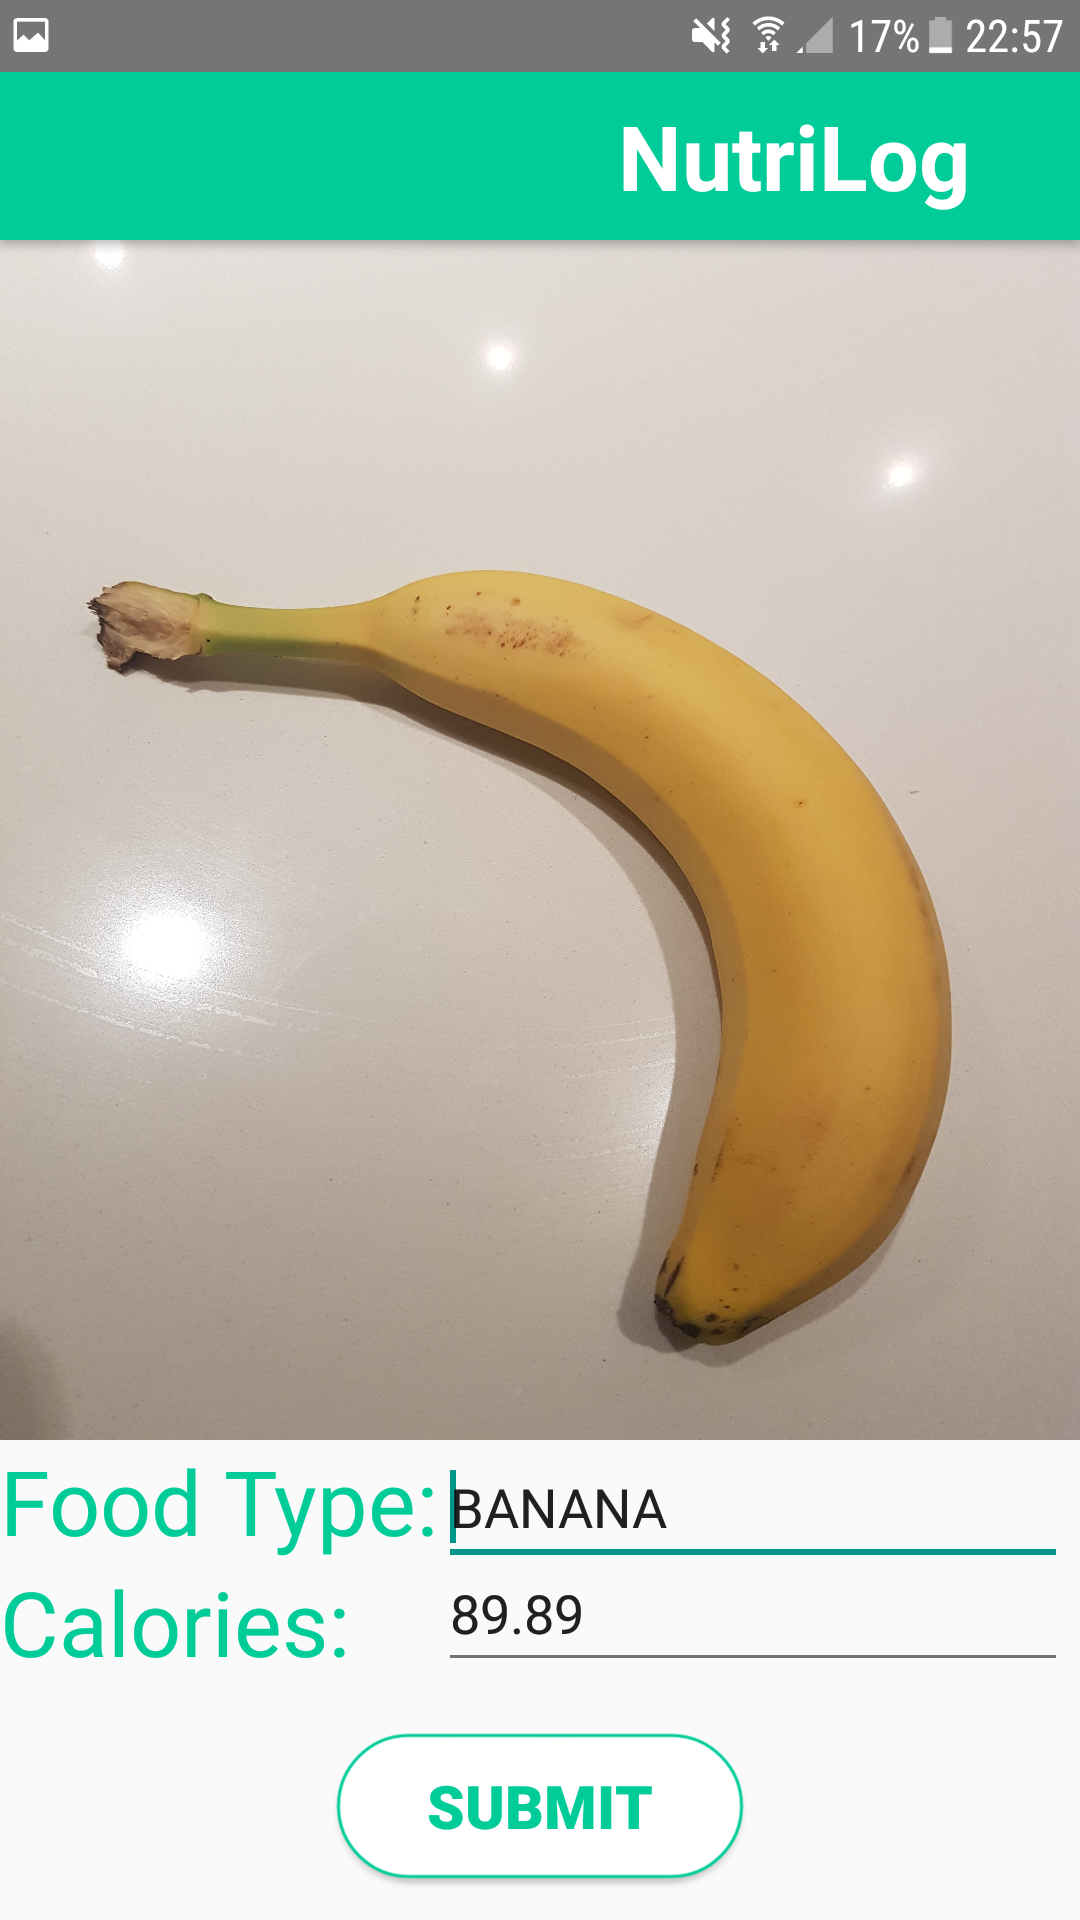
\includegraphics[width=.75\linewidth]{ui5} 
    \caption{Image Submit Activity} 
    \label{fig:ui5}
    \vspace{4ex}
  \end{minipage} 
\end{figure}

\begin{figure}
  \label{uiDesign2} 
  \begin{minipage}[b]{0.5\linewidth}
    \centering
    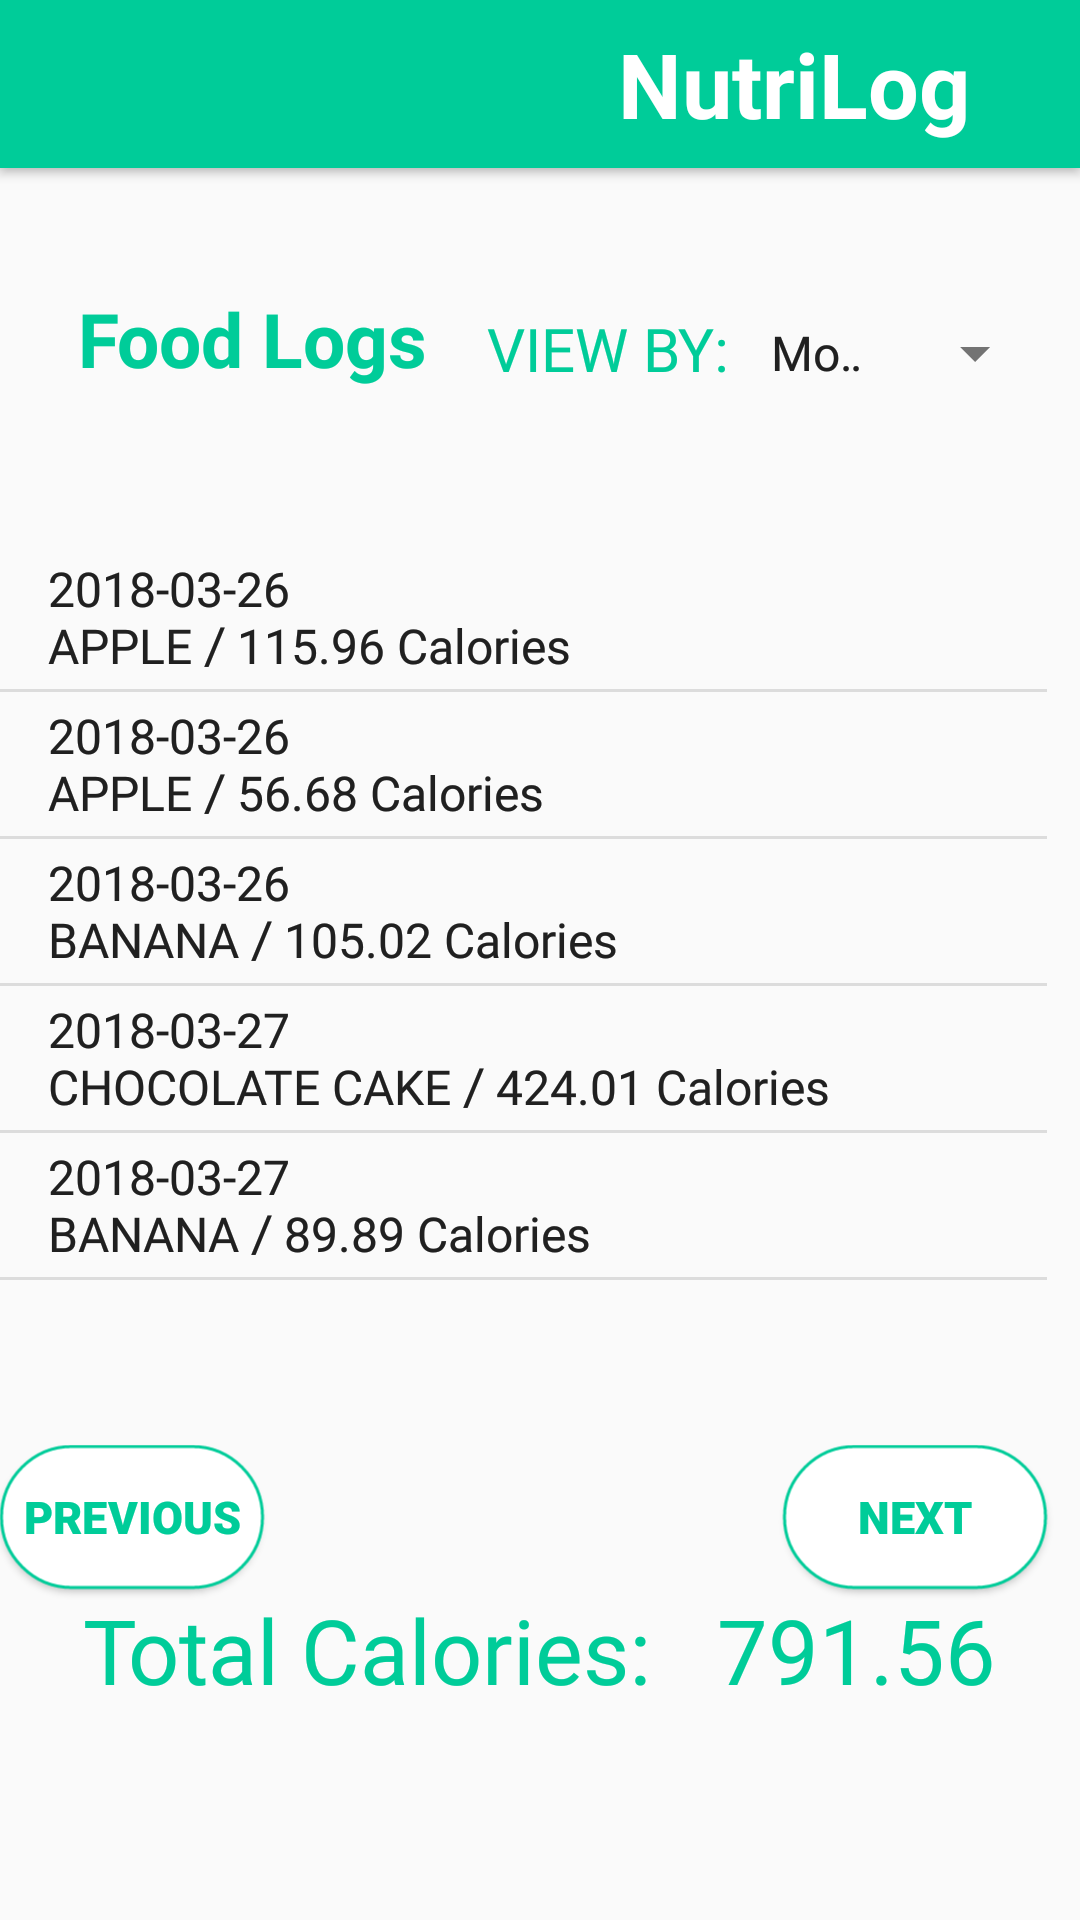
\includegraphics[width=.75\linewidth]{ui8} 
    \caption{FoodLog Month Activity} 
    \label{fig:ui8}
    \vspace{4ex}
  \end{minipage}
  \begin{minipage}[b]{0.5\linewidth}
    \centering
    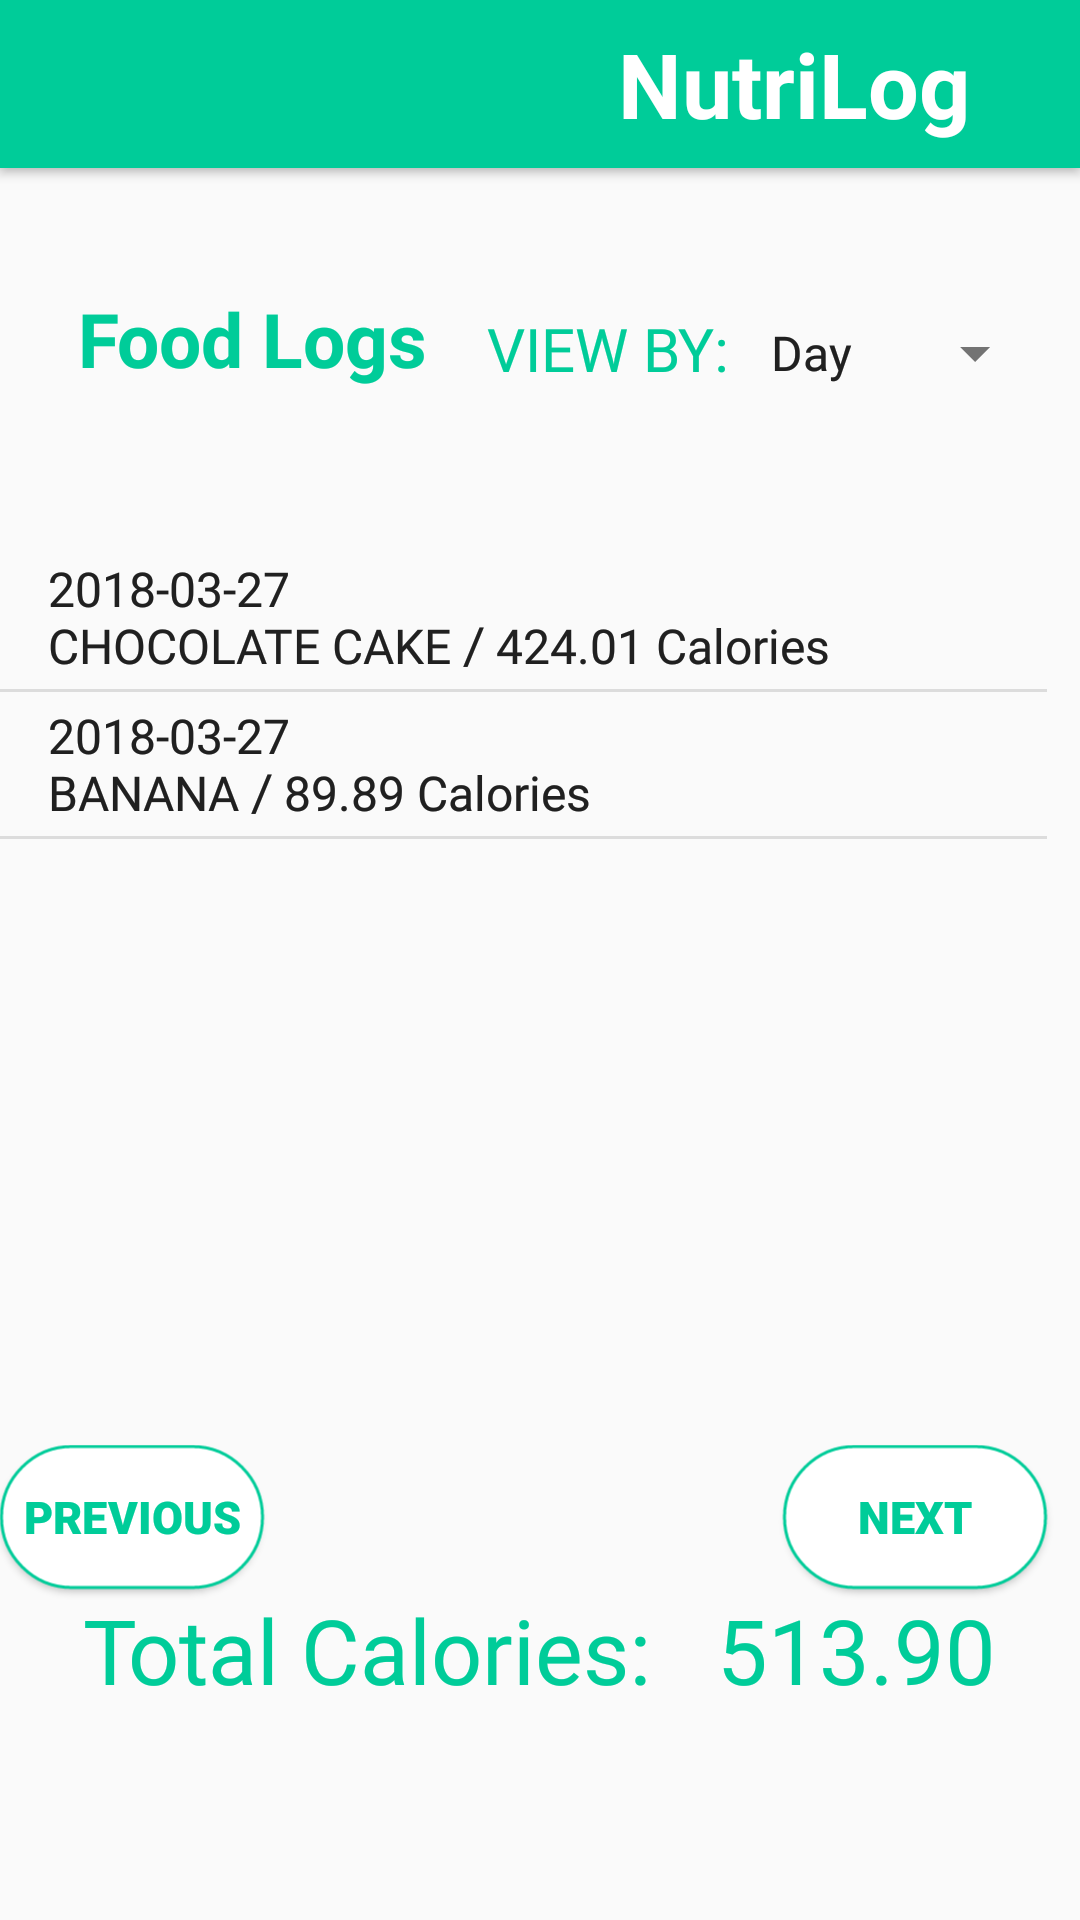
\includegraphics[width=.75\linewidth]{ui6} 
    \caption{FoodLog Day Activity} 
  \label{fig:ui6}
    \vspace{4ex}
  \end{minipage} 
  \begin{minipage}[b]{0.5\linewidth}
    \centering
    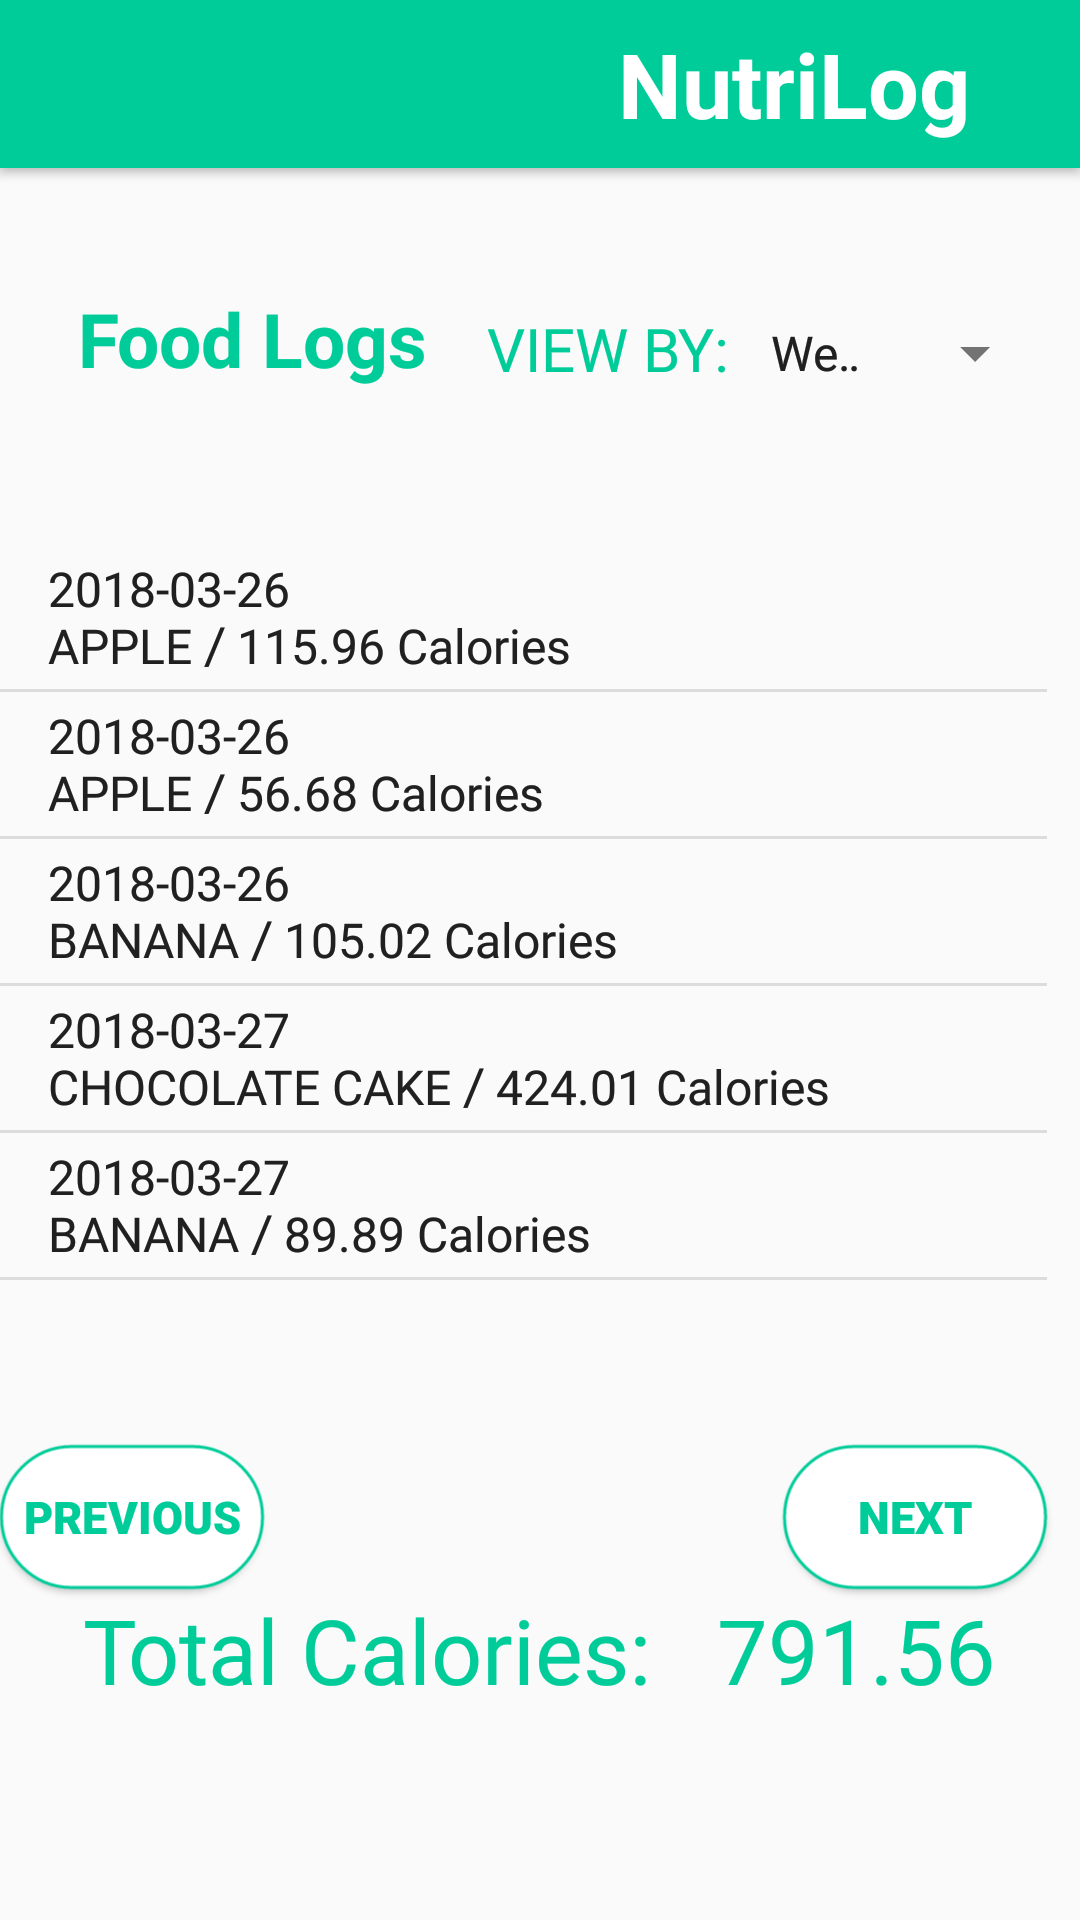
\includegraphics[width=.75\linewidth]{ui7} 
    \caption{FoodLog Week Activity} 
    \label{fig:ui7}
    \vspace{4ex}
  \end{minipage}%% 
  \begin{minipage}[b]{0.5\linewidth}
    \centering
    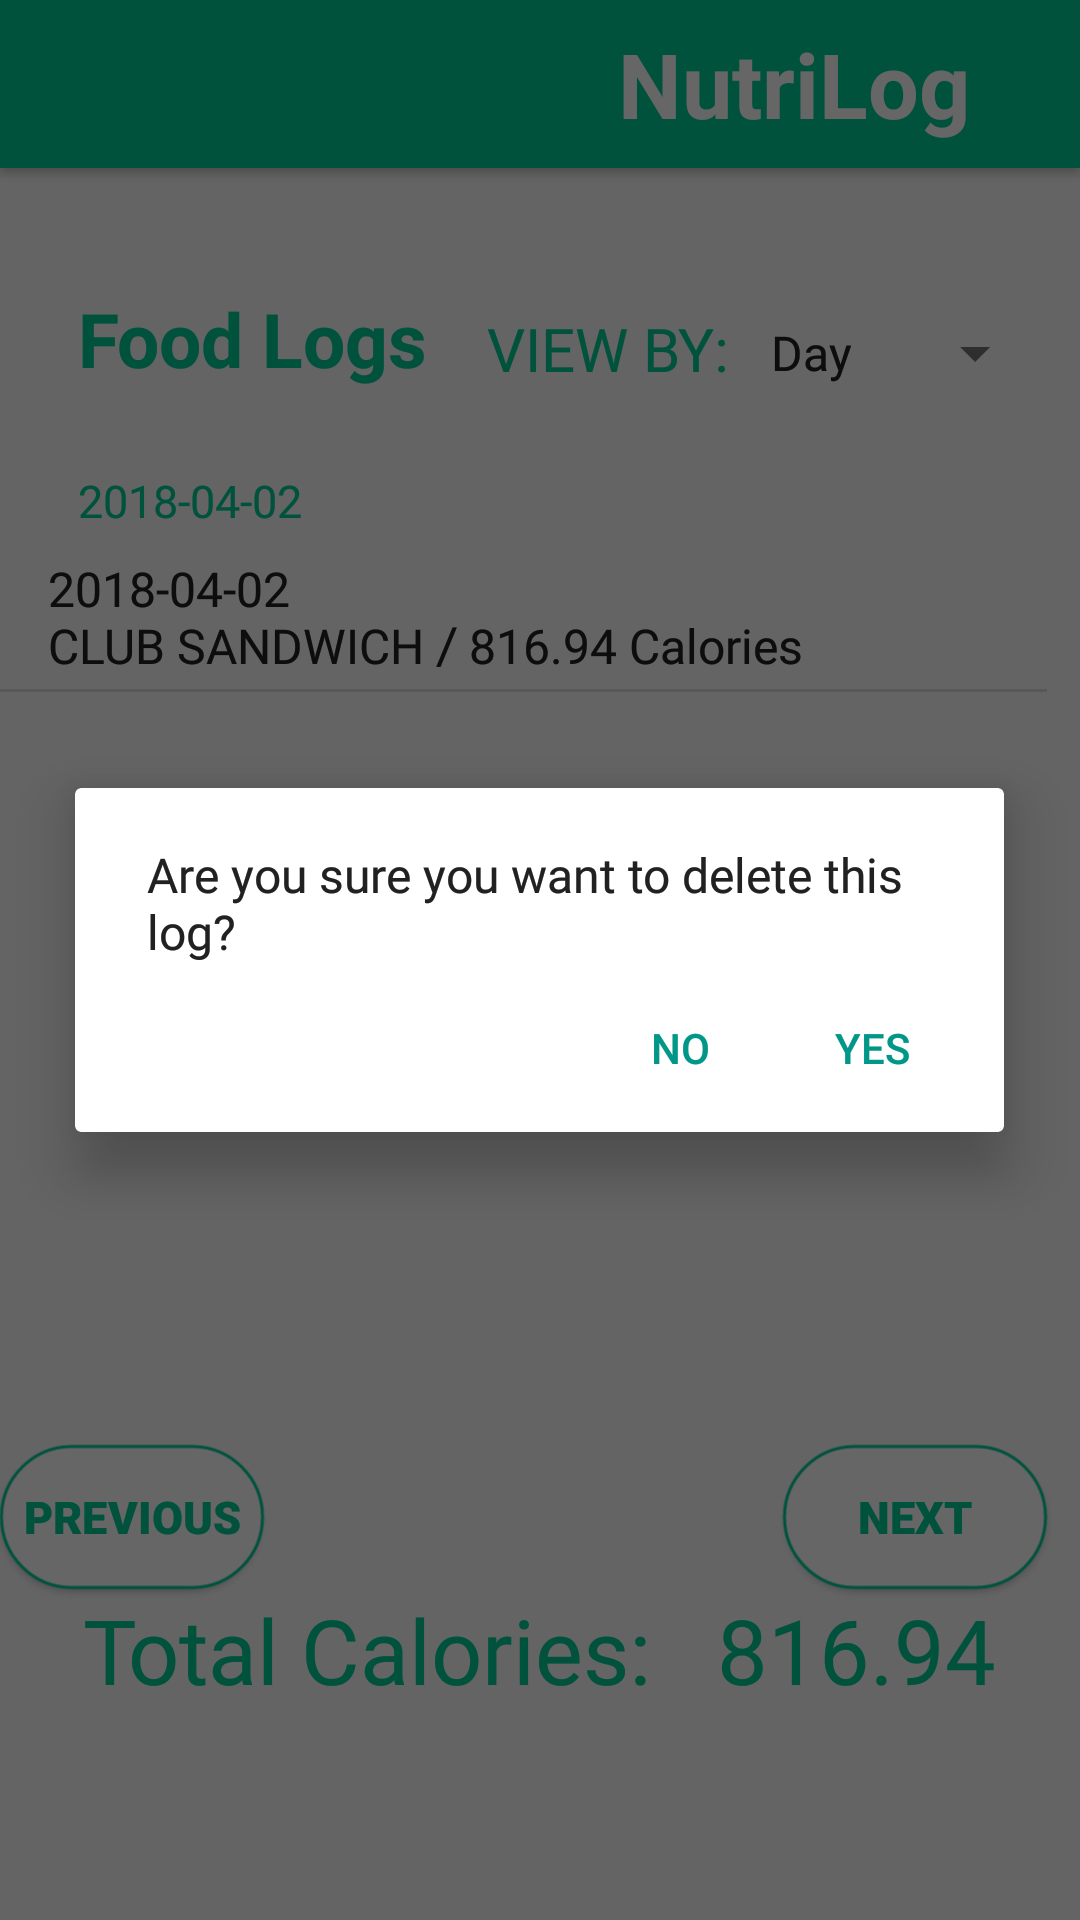
\includegraphics[width=.75\linewidth]{delete} 
    \caption{Food Log Deletion} 
  \label{fig:delete}
    \vspace{4ex} 
    \end{minipage}%% 
\end{figure}
\clearpage

\tocless\subsection{Technologies}

\tocless\subsubsection{Github}
Github was used as the version control backup system for this project.
Commit history can be seen in Figure \ref{fig:git}

\begin{figure}[h]
    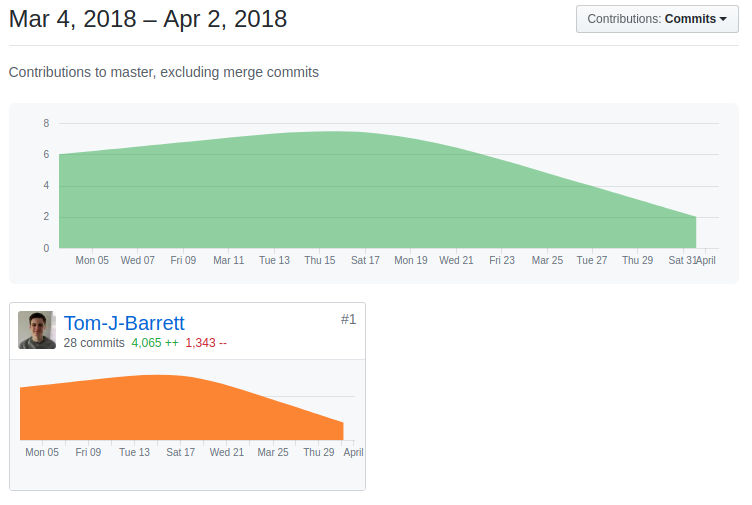
\includegraphics[scale=0.5]{git}
    \caption{Github Contributions to Master}
    \label{fig:git}
\end{figure}

\tocless\subsubsection{JSON}
JSON (JavaScript Object Notation) is a text format used to store data \parencite{json}.
It is both easy for machines to parse and for humans to read and write.
It is a data-interchange format as it is language independent.
JSON data structures as built on key pairs values and are normally parsed into arrays, lists or vectors.

\tocless\subsubsection{OkHttp}
OkHttp is a HTTP client created specifically for Java and Android applications \parencite{okhttp}.
It is a very efficient HTTP client with in built defense against troublesome networks (recovers from common problems silently).
Some of the efficiency components are as follows:
\begin{itemize}
    \item{HTTP/2 support}
    \item{Reduced request latency due to connection pooling}
    \item{Caching of responses}
\end{itemize}

\tocless\subsubsection{Nutritionix API}
The Nutritionix API is an API used to collect nutritional information \parencite{nutritionix}.
This project used this API to collect calorie information on a food item.
The free 'Hacker' account can support up to 10 active users.

\tocless\subsection{Software Quality Attributes}
Two main software quality attributed were focused on during the implementation of this prototype application. These were extensibility and maintainability.

Extensibility defines how easy it is to extend the functionality of the system.
There were certain places where the system developed is highly extensible.
A factory class was used to get the data access object that was used to store information in the application.
This factory class has a factory method that returns a DAO object which is an interface.
If the developer of the system needs to create an alternative way to store data in the application, they can create an object that implements the DAO interface and replace one line of code in the factory class.
A factpry class was also used to create a Host object with the same rationale.

Manitainability defines how easy it is to maintain a system.
The system is maintainable for many reasons.
These reasons include low coupling, high cohesion and readability.




